\documentclass[a4paper,fleqn, 10pt]{article}

\usepackage[utf8]{inputenc}
\usepackage[T1]{fontenc}
\usepackage[ngerman]{babel}
\usepackage[bottom=25mm,left=35mm,right=33mm,bottom=35mm]{geometry}
\usepackage{times}
\linespread{1.15}

\usepackage{turnthepage}
\renewcommand{\turnthepage}{\it bitte wenden}

\usepackage[pgfkeys,custom]{ati}
% \SetupExSheets{solution/print=true, question/type=exam}

\allowdisplaybreaks

\usepackage{import}

\usepackage{multicol}

\usepackage{dsfont}

\begin{document}

	\pagestyle{empty}

	\hrule
	\section*{\centering Mathematische Methoden der Physik I \\ Übungsserie 1: Aufgaben und Lösungen}
	\medskip
	Dr. Agnes Sambale \hfill Wintersemester 17/18\\
	% agnes.sambale@uni-jena.de \hfill Abgabe: Mittwoch, 01.11.17
	agnes.sambale@uni-jena.de
	\bigskip
	\hrule
	\bigskip
	\bigskip

	% \begin{atiTask}[
	title = Orthogonaltrajektorien und Richtungsfeld,
	language = Deutsch
]
	Betrachten Sie die Schar von Hyperbeln, die durch die folgende Gleichung beschrieben wird.
	Dabei stellt $c$ einen reellen Parameter dar.
	\[
		x^2 - 2y^2 = c^2
	\]
	\begin{atiSubtasks}
		\item{\locallabel{a}
			Stellen Sie eine Differentialgleichung auf, die diese Kurvenschar beschreibt.
		}
		\item{\locallabel{b}
			Leiten Sie daraus die Differentialgleichung für die zugehörigen Orthogonaltrajektorien her und skizzieren Sie deren Richtungsfeld.
		}
		\item{\locallabel{c}
			Lösen Sie die Differentialgleichung für die Orthogonaltrajektorien durch die Methode der Trennung der Variablen. Ergänzen Sie Ihre Skizze durch Hyperbeln und Orthogonaltrajektorien für den folgenden Anfangswert.
			\[
				x_0\define 6\separate y_0\define y(x_0)\define 4
			\]
		}
	\end{atiSubtasks}
\end{atiTask}
\begin{atiSolution}
	\begin{atiSubtaskSolutions}
		\item[\localref{a}]{
			Wir nehmen an, dass es sich bei $y$ um eine Funktion auf einer offenen Teilmenge $M\subset\setR$ handelt und dass der Graph von $y$ die gegebene Gleichung für alle $x\in M$ erfüllt.
			% In diesem Falle lässt sich die gegebene Gleichung für ein $x$ dieser offenen Teilmenge in der folgenden Form schreiben.
			\[
				x^2 - 2y^2(x) = c^2 \implies \fdrvopb{\tilde{x}}{\tilde{x}^2 - 2y^2(\tilde{x})}{x} = \fdrvopb{\tilde{x}}{c^2}{x} \implies 2x - 4y(x)y'(x) = 0
			\]
			Man erhält damit eine Differentialgleichung der folgenden Formen.
			\[
				2yy'=x \separate y'=\frac{x}{2y}\atiPoints[1]
			\]
		}
		\item[\localref{b}]{
			Die Orthogonaltrajektorien müssen demzufolge der folgenden Differentialgleichung genügen.
			Das Richtungsfeld dieser Differentialgleichung wird in der nachfolgenden Skizze abgebildet.
			\[
				y' = -\frac{2y}{x}\atiPoints[1]
			\]
		}
		\item[\localref{c}]{
			Durch Umstellung erhält man eine separierte Differentialgleichung, die sich für die Anfangswerte $x_0\in\setR\setminus\set{0}$ und $y_0\define y(0)\in\setR\setminus\set{0}$ direkt lösen lässt.
			\[
				\frac{y'(x)}{y(x)} = -\frac{2}{x} \implies \integral{x_0}{x}{\frac{y'(s)}{y(s)}}{s} = -2 \integral{x_0}{x}{\frac{1}{s}}{s}
			\]
			\[
				\implies \integral{y_0}{y(x)}{\frac{1}{s}}{s} = \ln\abs{\frac{y(x)}{y_0}} = \ln\curvb{\frac{y(x)}{y_0}} = -2 \ln\abs{\frac{x}{x_0}} = -2 \ln\curvb{\frac{x}{x_0}}
			\]
			\[
				\implies y(x) = \frac{y_0x_0^2}{x^2}\atiPoints[1]
			\]
			Setzt man nun $x_0 = 6$ und $y_0 = 4$, so erhält man die folgenden Aussagen.
			\[
				c^2 = x_0^2 - 2y_0^2 = 4 \implies c = \pm 2 \separate y_0x^2_0 = 144 \atiPoints[1]
			\]
			Auch hier sind die entsprechende Hyperbel und die, der Differentialgleichung entsprechenden, Orthogonaltrajektorie in der nachfolgenden Skizze eingezeichnet.
		}
		\begin{figure}[H]
			\center
			\atiPoints[3]
			\subimport{}{task-orthogonaltrajektorien_und_richtungsfeld-skizze}
			\caption*{Das Diagramm zeigt das Richtungsfeld der Orthogonaltrajektorien und das Beispiel einer zugehörigen Hyperbel.}
		\end{figure}
	\end{atiSubtaskSolutions}
\end{atiSolution}
	% \bigskip
	% \begin{atiTask}[
	title = Ähnlichkeitsdifferentialgleichung
]
	Gegeben sei eine gewöhnliche nicht-separable Differentialgleichung mit der freien Variable $t$ und der folgenden Form.
	Beachten Sie, dass $\timeDerivative{y}=\leibnizDerivative{y(t)}{t}$ die erste Ableitung nach der Zeit beschreibt.
	\[
		t\timeDerivative{y} = y\roundBrackets{1+\ln y - \ln t}
	\]

	Lösen Sie diese Differentialgleichung, indem Sie sie durch die folgende Substitution in eine separable Differentialgleichung überführen und überprüfen Sie Ihr Ergebnis, indem Sie eine Probe durchführen.
	\[
		z(t)\define\frac{y(t)}{t}\separate t\in\setReal^+
	\]
\end{atiTask}
\begin{atiSolution}
	Durch die Verwendung der Substitution lassen sich die folgenden Aussagen für alle $t\in\setReal^+$ treffen.
	\[
		y(t) = tz(t) \implies y'(t) = z(t) + tz'(t)\atiPoints[1]
	\]
	Das Umformen der ursprünglichen Differentialgleichung und Einsetzen der Substitution führt dann zur gewünschten separablen Differentialgleichung, die sich durch die Methode der Trennung der Variablen lösen lässt.
	\[
		ty'(t) = y(t)\boxBrackets{1+\ln \roundBrackets{\frac{y(t)}{t}}} \implies t\boxBrackets{z(t) + tz'(t)} = tz(t)\boxBrackets{1+\ln z(t)}
	\]
	\[
		\implies tz'(t) = z(t)\ln z(t) \implies \frac{z'(t)}{z(t)\ln z(t)} = \frac{1}{t}\atiPoints[1]
	\]
	\[
		\implies \integral{t_0}{t}{\frac{z'(s)}{z(s)\ln z(s)}}{s} = \integral{z_0}{z(t)}{\frac{1}{s\ln s}}{s} = \integral{t_0}{t}{\frac{1}{s}}{s}
	\]
	\[
		\implies \ln\roundBrackets{\frac{\ln z(t)}{\ln z_0}} = \ln \roundBrackets{\frac{t}{t_0}} \implies z(t) = \exp\roundBrackets{\frac{t\ln z_0 }{t_0}} = z_0^{\frac{t}{t_0}}\atiPoints[2]
	\]
	\[
		\implies y(t) = tz(t) = t\exp\roundBrackets{\frac{t\ln z_0 }{t_0}}\atiPoints[1]
	\]
	Für die Probe leitet man nun die Lösung ab und substituiert den erhaltenen Term mithilfe der berechneten Lösung.
	\[
		y'(t) = \exp\roundBrackets{\frac{t\ln z_0}{t_0}} + \frac{t\ln z_0}{t_0}\exp\roundBrackets{\frac{t\ln z_0}{t_0}}\atiPoints[\frac{1}{2}]
	\]
	\[
		\implies y'(t) = \frac{y(t)}{t} + \ln\roundBrackets{\frac{y(t)}{t}}\frac{y(t)}{t} = \frac{y(t)}{t}\boxBrackets{1 + \ln\roundBrackets{\frac{y(t)}{t}}}
	\]
	\[
		\implies ty'(t) = y(t)\boxBrackets{1+\ln\roundBrackets{\frac{y(t)}{t}}} = y(t)\boxBrackets{1 + \ln y(t) - \ln t}\atiPoints[\frac{1}{2}]
	\]
\end{atiSolution}
	% \newpage
	% \begin{atiTask}[
	title = Eine Zombieapokalypse,
	language = Deutsch
]
	Auf einer kleinen Insel gerät ein Virus in Umlauf, der die Bevölkerung in Zombies verwandelt.
	Jeder Infizierte hat in einer Zeitspanne $\tau\in\setReal^+$ Kontakt mit $\tau\cdot k$ anderen Personen, die teilweise ebenfalls infiziert, teilweise aber auch gesunde Menschen sind, wobei $k\in\setReal^+$ gilt.
	Gerät ein gesunder Mensch in Kontakt mit einem Zombie, so wird dieser infiziert.
	\medskip
	\begin{atiSubtasks}
		\item{\locallabel{a}
			Stellen Sie eine Differentialgleichung auf, die dieser Zombieapokalypse genügt.
			Verwenden Sie $N\in\setNatural$ für die Größe der Inselbevölkerung, $Z(t)\in[0,N]$ für die Anzahl der Infizierten, $M(t)\in[0,N]$ für die Anzahl der Gesunden und $t\in\setReal^+$ als freien Parameter der Zeit.

			\begin{atiNote}
				Betrachten Sie zunächst nur die Infizierten zum Zeitpunkt $t+\tau$ und überführen Sie die Differenzengleichung durch Grenzwertbildung in die gesuchte Differentialgleichung.
			\end{atiNote}
		}
		\item{\locallabel{b}
			Lösen Sie diese Differentialgleichung und das folgende Anfangswertproblem.
			\[
				t_0\define 0\separate Z_0\define Z(0) \define \frac{N}{21}
			\]
		}
		\item{\locallabel{c}
			Skizzieren Sie $Z(t)$ und $M(t)$ für $k=2$, $N=1050$ und $t\in\setReal^+$.
		}
		\item{\locallabel{d}
			\textbf{Zusatz:} Ab wann ist nur noch weniger als $1\appendUnit{\%}$ der Bevölkerung nicht infiziert?
			Wie beeinflussen die Parameter $k$ und $N$ diesen Zeitpunkt?
		}
	\end{atiSubtasks}
\end{atiTask}
\begin{atiSolution}
	\begin{atiSubtaskSolutions}
		\item[\localref{a}]{
			Wir definieren als Erstes den Anteil der gesunden Menschen $\alpha(t)\in[0,1]$ und den Anteil der infizierten Menschen $\beta(t)\in[0,1]$ für alle $t\in\setReal^+$.
			\[
				\alpha(t)\define \frac{M(t)}{N}\separate\beta(t)\define\frac{Z(t)}{N}
			\]
			Wir wählen nun eine festen Zeitpunkt $t\in\setReal^+$.
			Nähern wir für kleine Zeitspannen $\tau\in\setReal^+$ die Anzahl der Personen, die ein Zombie trifft, durch $\tau k$ an, so teilen sich Infizierte und Gesunde entsprechend ihrer Anteile auf diese Anzahl auf.
			% Trifft eine infizierte Person für kleine $\tau\in\setReal^+$ nun $\tau k$ andere Personen, so teilen sich Infizierte und Gesunde entsprechend ihrer Anteile $\alpha(t)$ und $\beta(t)$ auf diese Anzahl auf.
			\[
				\tau k \approx \tau k\alpha(t) + \tau k\beta(t)
			\]
			Die Anzahl $S(t)$ der gesunden Menschen, die ein Zombie in der Zeitspanne $\tau$ trifft und infiziert, kann demnach wie folgt für kleine $\tau$ approximiert werden.
			\[
				S(t) \approx \tau k \alpha(t) = \frac{\tau k}{N} M(t)
			\]
			Diese Approximation gilt für jeden Zombie.
			Dementsprechend lässt sich nun die Anzahl der Zombies $Z(t+\tau)$ nach der Zeitspanne $\tau$ beschreiben.
			% Damit ergibt sich die Gesamtanzahl $\Delta Z(t)$ der gesunden Menschen, die während dieser Zeitspanne $\tau$ infiziert werden, durch eine Multiplikation von $S(t)$ mit der Anzahl aller Zombies $Z(t)$.
			% \[
			% 	\Delta Z(t) = S(t)Z(t) = \tau k\alpha(t)Z(t) = \frac{\tau k}{N}M(t)Z(t) = \frac{\tau k}{N} \boxBrackets{N-Z(t)}Z(t)
			% \]
			\[
				Z(t+\tau) \approx Z(t) + S(t)Z(t) = Z(t) + \frac{\tau k}{N} \boxBrackets{N-Z(t)}Z(t)\atiPoints[1]
			\]
			\[
				\implies \frac{Z(t+\tau)-Z(t)}{\tau} \approx \frac{k}{N}\boxBrackets{N-Z(t)}Z(t)
			\]
			Um die Fehler der Näherung mithilfe einer Differentialgleichung zu korrigieren, bildet man den Grenzwert der erhaltenen Differenzengleichung für $\tau\conv 0$.
			\[
				Z'(t) = \lim_{\tau\conv 0}\frac{Z(t+\tau)-Z(t)}{\tau} = \frac{k}{N}\boxBrackets{N-Z(t)}Z(t)
			\]
			\[
				\implies Z' = \frac{k}{N}(N-Z)Z \atiPoints[1]
			\]
		}
		\item[\localref{b}]{
			Bei der oben beschriebenen Gleichung handelt es sich offensichtlich um eine separable Differentialgleichung.
			Die Methode der Trennung der Variablen ergibt dann das Folgende.
			\[
				\frac{Z'(t)}{\boxBrackets{N-Z(t)}Z(t)} = \frac{k}{N} \implies \integral{t_0}{t}{\frac{Z'(s)}{\boxBrackets{N-Z(s)}Z(s)}}{s} = \integral{t_0}{t}{\frac{k}{N}}{s}
			\]
			\[
				\implies \integral{Z_0}{Z(t)}{\frac{1}{(N-s)s}}{s} = \frac{k}{N}(t-t_0)\atiPoints[1]
			\]
			Für die Lösung des Integrals zeigt sich eine Partialbruchzerlegung als sinnvoll.
			\[
				\frac{1}{(N-s)s} = \frac{N}{N}\frac{1}{(N-s)s} = \frac{1}{N}\frac{N-s+s}{(N-s)s} = \frac{1}{Ns} - \frac{1}{N(s-N)}
			\]
			\[
				\implies \integral{Z_0}{Z(t)}{\frac{1}{(N-s)s}}{s} = \integral{Z_0}{Z(t)}{\frac{1}{Ns}}{s} - \integral{Z_0}{Z(t)}{\frac{1}{N(s-N)}}{s}
			\]
			\[
				= \frac{1}{N}\ln\boxBrackets{\frac{Z(t)}{Z_0}} - \frac{1}{N}\ln\boxBrackets{\frac{Z(t)-N}{Z_0-N}} = \frac{1}{N}\ln\roundBrackets{\frac{Z(t)\boxBrackets{Z_0-N}}{Z_0\boxBrackets{Z(t)-N}}}\atiPoints[+1]
			\]
			Die Lösung des Integrals wird nun eingesetzt und die entstehende Gleichung wird explizit nach $Z(t)$ umgestellt.
			\[
				\frac{Z(t)}{Z(t)-N} = \frac{Z_0e^{k(t-t_0)}}{Z_0-N} = -Ae^{k(t-t_0)}\separate A\define \frac{Z_0}{N-Z_0}
			\]
			\[
				\implies Z(t) = \frac{NAe^{k(t-t_0)}}{1 + Ae^{k(t-t_0)}} = N\roundBrackets{1 - \frac{1}{1+Ae^{k(t-t_0)}}}\atiPoints[1]
			\]
			Nun setzen wir die Anfangswerte ein und unterstreichen unser Ergebnis doppelt.
			\[
				A = \frac{1}{20} \implies Z(t) = N\roundBrackets{1 - \frac{1}{1+\frac{1}{20}e^{kt}}}\atiPoints[1]
			\]
		}
		\item[\localref{c}]{
			Die nachfolgende Skizze zeigt die Werte $M(t)$ und $Z(t)$ für verschiedene Zeiten $t\in\setReal^+$.
		}
		\item[\localref{d}]{
			Es sei $\alpha^*\in\roundBrackets{0,1-\frac{Z_0}{N}}$ eine feste Grenze für den Anteil der Menschen.
			Wir suchen nun den frühesten Zeitpunkt $t^*\in\setReal^+$, sodass $\alpha(t^*)\leq\alpha^*$ gilt.
			Durch Äquivalenzumformungen zeigt man, dass $t^*$ existiert und eindeutig ist.
			\[
				\alpha^* = \alpha(t^*) = 1-\beta(t^*) = 1 - \frac{Z(t^*)}{N} = \frac{1}{1 + Ae^{k(t^*-t_0)}}
			\]
			\[
				\implies t^* = t_0 + \frac{1}{k}\ln\boxBrackets{\frac{1}{A}\roundBrackets{\frac{1}{\alpha^*}-1}} = t_0 + \frac{1}{k}\ln\boxBrackets{\frac{N-Z_0}{Z_0}\roundBrackets{\frac{1}{\alpha^*}-1}}
			\]
			Setzt man nun die gewünschten Werte der Parameter ein, so erhält man das folgende Ergebnis.
			\[
				t_0 = 0\separate k=2\separate A = 0.05 \separate\alpha^* = 1\appendUnit{\%}\implies t^* = \frac{\ln 1980}{2} \approx 3.8\atiPoints[+1]
			\]
			Zu beachten ist, dass $t^*$ sowohl von $k$ als auch von $N$ abhängig ist.
			Steigt $k$, so verringert sich $t^*$.
			Steigt $N$, so erhöht sich auch $t^*$.\atiPoints[+1]
		}
	\end{atiSubtaskSolutions}
	\begin{figure}[H]
		\center
		\atiPoints[2]
		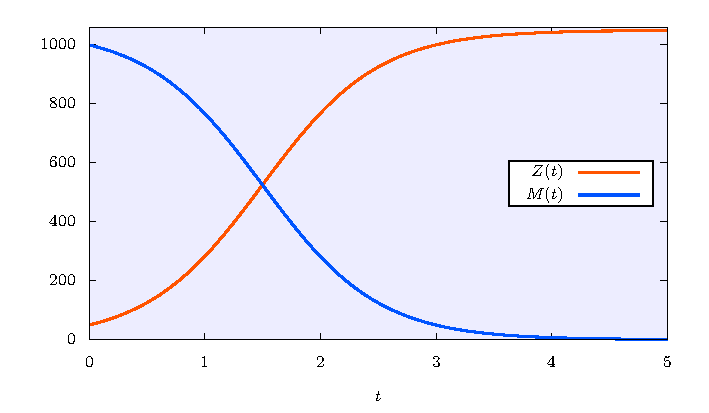
\includegraphics[width=0.9\textwidth]{task-eine_zombieapokalypse-diagram}
		\caption{Die Abbildung zeigt die Anzahl der Zombies $Z(t)$ und der gesunden Menschen $M(t)$ für verschiedene Zeiten $t$.}
	\end{figure}
\end{atiSolution}

	\begin{atiTask}[
	title = Klassifikation von gewöhnlichen Differentialgleichungen
]
	Klassifizieren Sie die folgenden gewöhnlichen Differentialgleichungen durch ihre Ordnung, Homogenität, Linearität und Separabilität.
	Lösen Sie zudem die separablen Differentialgleichungen.
	\begin{atiSubequations}
	\begin{multicols}{2}
		\item{\locallabel{dgl1}
			\leibnizNDerivative[2]{y(x)}{x} + 2\leibnizDerivative{y(x)}{x} = y
		}
		\item{\locallabel{dgl2}
			\leibnizDerivative{y(x)}{x} + \sin y - x^2 = 0
		}
		\item{\locallabel{dgl3}
			y' + \tan(x)\cdot y = 0
		}
		\item{\locallabel{dgl4}
			\frac{y''}{y'} + x = 0
		}
		\item{\locallabel{dgl5}
			yy'-x = 0
		}
		\item{\locallabel{dgl6}
			\frac{x+1}{y+2} = \leibnizDerivative{y(x)}{x}
		}
	\end{multicols}
		\item{\locallabel{dgl7}
			\sqrt{y^2 + 3a^2 + ya\roundBrackets{2-\frac{4a}{2y}}} + \leibnizDerivative{y(x)}{x}\sqrt{x^2-a^2} = \sqrt{x+a}
		}
	\end{atiSubequations}
\end{atiTask}
\begin{atiSolution}
	\begin{atiSubtaskSolutions}
		\item[\localref{dgl1}]{
			Durch eine einfache Umformung erhalten wir die folgende Differentialgleichung.
			\[
				y'' + 2y' -y = 0
			\]
			\atiPoints[1]Damit handelt es sich bei dieser Differentialgleichung um eine gewöhnliche, lineare, homogene, nicht-separable Differentialgleichung 2.Ordnung.
		}
		\item[\localref{dgl2}]{
			Durch eine einfache Umformung erhalten wir die folgende Differentialgleichung.
			\[
				y'+ \sin y = x^2
			\]
			\atiPoints[1]Damit handelt es sich bei dieser Differentialgleichung um eine gewöhnliche, nicht-lineare, nicht-separable Differentialgleichung 1.Ordnung.
		}
		\item[\localref{dgl3}]{
			Durch eine Äquivalenzumformung lässt sich die Differentialgleichungen in die beiden folgenden Formen bringen.
			\[
				y' + \tan (x)y = 0 \separate y' = -y\tan x
			\]
			\atiPoints[1]Damit handelt es sich bei dieser Differentialgleichung um eine gewöhnliche, lineare, homogene, separable Differentialgleichung 1.Ordnung.
			Durch Anwendung der Methode der Trennung der Variablen, erhält man dann die folgende Lösung.
			\[
				\frac{y'(x)}{y(x)} = -\tan x \implies \integral{y_0}{y}{\frac{1}{s}}{s} = \integral{x_0}{x}{-\tan s}{s}
			\]
			\[
				\implies \ln\absolute{\frac{y(x)}{y_0}} = \ln\absolute{\frac{\cos x}{\cos x_0}} \implies \absolute{y(x)} = \absolute{\frac{y_0}{\cos x_0}} \absolute{\cos x}\atiPoints[1]
			\]
		}
		\item[\localref{dgl4}]{
			Wir formen wieder die gegebene Differentialgleichung um und erhalten die folgenden beiden Ausdrücke.
			\[
				y'' = -xy' \separate y'' + xy' = 0
			\]
			\atiPoints[1]Damit handelt es sich bei dieser Differentialgleichung um eine gewöhnliche, lineare, homogene, nicht-separable Differentialgleichung 2.Ordnung.
			\atiPoints[+\frac{1}{2}]Durch die Substitution mit $z\define y'$ lässt sich zudem noch zeigen, dass sie in eine separable Differentialgleichung umgeformt werden kann.
		}
		\item[\localref{dgl5}]{
			\atiPoints[1]Es handelt sich um eine gewöhnliche, nicht-lineare, separable Differentialgleichung 1.Ordnung.
			Es lässt sich hier keine Homogenität definieren, da sie nicht linear ist.
			Die Methode der Trennung der Variablen liefert dann die folgende Lösung.
			\[
				\integral{x_0}{x}{y(s)y'(s)}{s} = \integral{x_0}{x}{s}{s} \implies \integral{y_0}{y(x)}{s}{s} = \frac{y^2(x)- y^2_0}{2} = \frac{x^2-x_0^2}{2}
			\]
			\[
				\implies y^2(x) = x^2 - x_0^2 + y_0^2 \implies y(x) = \pm\sqrt{x^2-x_0^2+y_0^2}\atiPoints[1]
			\]

		}
		\item[\localref{dgl6}]{
			Durch die Trennung von Zähler und Nenner lässt sich die Differentialgleichung in eine Form bringen, an der sich ihre Eigenschaften ablesen lassen.
			\[
				y' = (x+1)\frac{1}{y+2}
			\]
			\atiPoints[1]Es handelt sich um eine gewöhnliche, nicht-lineare, separable, Differentialgleichung 1.Ordnung.
			Die Methode der Trennung der Variablen liefert dann die folgende Lösung.
			\[
				\boxBrackets{y(x)+2}y'(x) = x+1 \implies \integral{y_0}{y(x)}{s+2}{s} = \integral{x_0}{x}{s+1}{s}
			\]
			\[
				\implies \frac{1}{2}\roundBrackets{\boxBrackets{y(x)+2}^2 - \boxBrackets{y_0 + 2}^2} = \frac{1}{2}\roundBrackets{(x+1)^2 - (x_0+1)^2}
			\]
			\[
				\implies \boxBrackets{y(x)+2}^2 = (x+1)^2 - (x_0+1)^2 + \roundBrackets{y_0+2}^2
			\]
			\[
				\implies y(x) = -2 \pm \sqrt{(x+1)^2 - (x_0+1)^2 + \roundBrackets{y_0+2}^2}\atiPoints[1]
			\]
		}
		\item[\localref{dgl7}]{
			Berechnet man den ersten Term auf der linken Seite dieser Gleichung, so ist es möglich die zweite binomische Formel zu verwenden.
			In diesem Falle erhält man das folgende Resultat.
			\[
				\absolute{y+a} + y'\sqrt{x^2-a^2} = \sqrt{x+a}
			\]
			\atiPoints[1]Damit handelt es sich bei dieser Differentialgleichung um eine gewöhnliche, nicht-lineare, nicht-separable Differentialgleichung 1.Ordnung.
		}
	\end{atiSubtaskSolutions}
\end{atiSolution}
	\newpage
	\begin{atiTask}[
	title = Zwei separable Differentialgleichungen,
	language = Deutsch
]
	Lösen Sie die folgenden Differentialgleichungen mittels Trennung der Variablen.
	Überprüfen Sie Ihr Ergebnis, indem Sie die Probe durch Einsetzen Ihrer Lösung in die ursprüngliche Differentialgleichung durchführen.
	\begin{atiSubequations}
		% \medskip
		% \begin{minipage}[t]{0.5\textwidth}
		% \begin{multicols}{2}
		\item{
			\frac{1}{\cos x}\fdrv{y(x)}{x} = -\tan x \cdot y^{-2}
		}
		% \end{minipage}
		% \begin{minipage}{0.5\textwidth}
		\item{
			xyy' = y-1
		}
		% \end{minipage}
		% \end{multicols}
	\end{atiSubequations}
\end{atiTask}

	% \begin{atiTask}[
	topic = Gewöhnliche Differentialgleichungen,
	subtopic = Separable Differentialgleichungen,
	title = Homogene Differentialgleichungen,
	language = Deutsch
]
	Eine Funktion von zwei Variablen heißt homogen vom Grad $k$, wenn für einen beliebigen Parameter $\lambda$ das Folgende gilt.
	\[
		f(\lambda x, \lambda y) = \lambda^k f(x,y)
	\]
	Dementsprechend nennt man eine Differentialgleichungen der folgenden Form auch homogen, wenn $f$ und $g$ homogene Funktionen vom gleichen Grad sind.
	\[
		y' = \frac{f(x,y)}{g(x,y)}
	\]

	\begin{atiSubtasks}
		\item \label{subtask:homogene-differentialgleichung-a}
		Lösen Sie die folgende homogene Differentialgleichung.
		\[
			2xyy^\prime = 3y^2 - x^2
		\]
		Anleitung: Führen Sie eine neue Variable $z(x)$ gemäß $y(x)\definedby x\cdot z(x)$ ein und behandeln Sie die für $z(x)$ entstehende Differentialgleichung mit der Methode der Trennung der Variablen.

		\item
		Lösen Sie die folgende Differentialgleichung, die nicht homogen ist.
		\[
			y^\prime = \frac{y+x-2}{y-x+4}
		\]
		Schuld daran sind die beiden additiven Konstanten in Zähler und Nenner des Bruches auf der rechten Seite.
		Gehen Sie in zwei Schritten nach folgender Anleitung vor.
		\begin{atiItems}
			\item Führen Sie die neue Variablen $v\define y-y_0$ und $u\define x-x_0$ ein und bestimmen Sie $x_0$ und $y_0$, sodass die neue Differentialgleichung in den Variablen $u$ und $v$ homogen ist (Gleichungssystem mit zwei Unbekannten).

			\item Verfahren Sie mit der Substitution $v(u)\definedby u\cdot z(u)$ weiter, wie in Teilaufgabe \ref{subtask:homogene-differentialgleichung-a}.
		\end{atiItems}

		\item
		Machen Sie in beiden Fällen die Probe durch Einsetzen Ihrer Lösung $y(x)$ in die ursprüngliche Differentialgleichung.
	\end{atiSubtasks}
\end{atiTask}
% \begin{atiSolution}

% \end{atiSolution}
	% \begin{atiTask}[
	topic = Gewöhnliche Differentialgleichungen,
	subtopic = Separable Differentialgleichungen,
	title = Orthogonaltrajektorien,
	language = Deutsch
]
	\begin{atiSubtasks}
		\item {
			Skizzieren Sie die folgende Kurvenschar, wobei $c$ eine eine reelle Konstante darstellt.
			\[
				xy = c
			\]
			Bestimmen Sie dazu die Schar der Orthogonaltrajektorien ud tragen Sie diese in Ihre Skizze ein.
		}
		\item{
			Skizzieren Sie die folgende Kurvenschar und bestimmen Sie die Differentialgleichung, die dieser Kurvenschar genügt.
			Auch hier stellt $c$ eine reelle Konstante dar.
			\[
				y^2 = 4c(x+c)
			\]
			Zeigen Sie dann, dass diese Differentialgleichung die gleiche bleibt, wenn $y'$ durch $-\frac{1}{y'}$ ersetzt wird.
			Welche Schlussfolgerungen ziehen Sie aus dieser Eigenschaft?
		}
	\end{atiSubtasks}
\end{atiTask}
	% \begin{atiTask}[
	topic = Gewöhnliche Differentialgleichungen,
	subtopic = Separable Differentialgleichungen,
	title = Die Methode der Variablentrennung,
	language = deutsch,
]
	Lösen Sie die folgenden Differentialgleichungen durch Trennung der Variablen und bestimmen Sie gegebenenfalls die Integrationskonstante, sodass die nebenstehenden Anfangsbedingungen erfüllt sind.
	\begin{atiSubequations}
		\item{
			\label{dgl-1}
			y' = \frac{x e^{-y}}{x^2 + 1} \separate y(1) = 0
		}
		\item{
			\label{dgl-2}
			xyy' = \frac{x^2 + 2}{y-1}
		}
		\item{
			\label{dgl-3}
			y' = \frac{x+y}{x+y+2} \separate y(1) = -1
		}
	\end{atiSubequations}
	Machen Sie in allen Fällen die Probe durch Einsetzen Ihrer Lösung in die ursprüngliche Differentialgleichung. Dies ist auch dann verlangt, wenn die Lösung nur in impliziter Form angebbar ist.

	\begin{atiNote}
		Führen Sie in Teilaufgabe \ref{dgl-3} die neue Variable $z(x)\define x + y(x)$ ein.
	\end{atiNote}
\end{atiTask}

\begin{atiSolution}
	\begin{atiSubtaskSolutions}
		\item[\ref{dgl-1}]{
			Separieren Sie $x$ und $y(x)$ auf jeweils eine Seite der Differentialgleichung und integrieren Sie die erhaltene Gleichung.
			\[
				y'(x) = \frac{xe^{-y(x)}}{x^2 + 1} \implies e^{y(x)} y'(x) = \frac{x}{x^2 + 1}
			\]
			\[
				\implies \integral{}{}{e^{y(x)}y'(x)}{x} = \integral{}{}{\frac{x}{x^2+1}}{x}
				\atiPoints[1]
			\]
			Lösen Sie das Integral mithilfe einer logarithmischen Integration oder durch Substitution, indem Sie $x^2$ durch eine geeignete Variable ersetzen.
			\[
				\integral{}{}{e^y}{y} = \frac{1}{2} \integral{}{}{\frac{2x}{x^2+1}}{x}
			\]
			\[
				\implies e^{y(x)} = \frac{1}{2}\ln(x^2 + 1) + C = \ln\sqrt{x^2 + 1} + C
				\atiPoints[1]
			\]
			Notieren Sie die explizite Lösung durch die Anwendung von $\ln$.
			\[
				y(x) = \ln\boxb{\ln\curvb{A\sqrt{x^2+1}}} \separate A\define e^C
				\atiPoints[1]
			\]
			Fordern Sie nun $y(1)\demand 0$, bestimmen Sie die Konstante $A$ und setzen Sie die erhaltene Lösung in die explizite allgemeine Form ein.
			\[
				y(1) \demand 0 \implies 1 = \ln \curvb{A\sqrt{2}} \implies A = \frac{\sqrt{2}}{2}e
				\atiPoints[1]
			\]
			\[
				y(x) = \ln\boxb{\ln\curvb{\frac{e}{2}\sqrt{2(x^2 + 1)}}} = \ln\boxb{1 + \ln\curvb{\frac{1}{2}\sqrt{2(x^2+1)}}}
				\atiPoints[1]
			\]

			Sei $y\definedby \ln u$ mit $u(x) = \ln\curvb{A\sqrt{x^2+1}}$.
			Dann erhält man durch die Anwendung der Kettenregel die folgende Aussage.
			\[
				y'(x) = u'(x) \ln' u(x) = \frac{1}{A\sqrt{x^2+1}} \cdot A \cdot \frac{2x}{2\sqrt{x^2+1}} \cdot \frac{1}{u(x)} = e^{-y(x)} \frac{x}{x^2+1}
				\atiPoints[1]
			\]
		}

		\item[\ref{dgl-2}]{
			Separieren Sie $x$ und $y(x)$ wieder auf jeweils eine Seite der Differentialgleichung
			\[
				xy(x)y'(x) = \frac{x^2+2}{y(x)-1} \implies y(x)\boxb{y(x)-1}y'(x) = \frac{x^2+2}{x}
				\atiPoints[1]
			\]
			Integrieren Sie die rechte Seite der erhaltenen Gleichung durch Polynomintegration und der Umkehrregel.
			\[
				\integral{}{}{\boxb{y^2(x)-y(x)}y'(x)}{x} = \integral{}{}{\curvb{x+\frac{2}{x}}}{x}
			\]
			\[
				\implies \integral{}{}{y^2-y}{y} = \frac{x^2}{2} + 2\ln\abs{x}
				\atiPoints[1]
			\]
			Lösen Sie nun auch das Integral der rechten Seite durch Polynomintegration und notieren Sie die allgemeine Lösung in impliziter Form.
			\[
				\frac{y^3}{3} - \frac{y^2}{2} = \frac{x^2}{2} + 2\ln\abs{x} + C
			\]
			\[
				\implies 2y^3 - 3y^2 = 3x^2 + 12 \ln \abs{x} + D
				\atiPoints[1]
			\]

			Durch implizite Ableitung der allgemeinen Form erhalten Sie Folgendes.
			\[
				6y^2(x)y'(x) - 6y(x)y'(x) = 6x + \frac{12}{x} \implies y(x)\boxb{y(x)-1}y'(x) = x + \frac{2}{x}
			\]
			\[
				\implies xy(x)\boxb{y(x)-1}y'(x) = x^2+2
				\atiPoints[1]
			\]
		}

		\item[\ref{dgl-3}]{
			Definieren Sie $z(x)\define x + y(x)$ und bestimmen Sie die Ableitung von $z$.
			\[
				z'(x) = 1 + y'(x) \implies y'(x) = z'(x) - 1
			\]
			Substituieren Sie nun $x+y(x)$ in der Differentialgleichung durch $z(x)$.
			\[
				y'(x) = \frac{x+y(x)}{x+y(x)+2} \implies z'(x) - 1 = \frac{z}{z+2}
				\atiPoints[1]
			\]
			Führen Sie für die erhaltene Differentialgleichung das Verfahren der Trennung der Variablen durch.
			Separieren Sie $z(x)$ und $x$ auf jeweils eine Seite und integrieren Sie die erhaltene Gleichung.
			\[
				z'(x) = \frac{z(x)}{z(x)+2} + 1 = \frac{2z(x)+2}{z+2} = 2\,\frac{z(x)+1}{z(x)+2}
				\atiPoints[1]
			\]
			\[
				\implies \integral{}{}{\frac{z(x)+2}{z(x)+1}z'(x)}{x} = \integral{}{}{\curvb{1 + \frac{1}{z+1}}}{z} = \integral{}{}{2}{x}
			\]
			\[
				\implies z(x) + \ln\abs{z(x)+1} = 2x + C
				\atiPoints[1]
			\]
			Führen Sie die Resubstitution durch und geben Sie die allgemeine Lösung in impliziter Form an.
			\[
				x + y(x) + \ln\abs{x+ y(x) + 1} = 2x + C
			\]
			\[
				\implies x+y(x)+1 = \exp(x-y(x)+C) = Ae^{x-y(x)} \separate A\define e^C
			\]
			\[
				\implies x+y(x) = Ae^{x-y(x)} -1
				\atiPoints[1]
			\]
			Fordern Sie die gegebenen Anfangsbedingungen und bestimmen Sie die Konstante $A$.
			\[
				y(1)\demand -1 \implies 0=Ae^2-1 \implies A= e^{-2}
			\]
			\[
				\implies x+y(x) = \frac{e^{x-y(x)}}{e^2}-1 = e^{x-y(x)-2}-1
				\atiPoints[1]
			\]

			Auch hier ist wieder eine implizite Ableitung notwendig.
			\[
				1+y'(x) = Ae^{x-y(x)} \boxb{1-y'(x)}
			\]
			Durch Verwendung der allgemeinen Lösung erhalten Sie für die Konstante $A$ den folgenden Ausdruck.
			\[
				A = e^{y(x)-x}\boxb{x+y(x)+1}
			\]
			Das Einsetzen dieser Gleichung resultiert dann in der gewünschten Differentialgleichung.
			\[
				1+y'(x) = e^{y(x)-x}\boxb{x+y(x)+1} e^{x-y(x)} \boxb{1-y'(x)}
			\]
			\[
				\implies 1+y'(x) = x+y(x)+1 - \boxb{x+y(x)+1}y'(x)
			\]
			\[
				\implies y'(x)\boxb{x+y(x)+2} = x+y(x)
				\atiPoints[1]
			\]
		}
	\end{atiSubtaskSolutions}
\end{atiSolution}

	% \begin{atiTask}[
	title = Die Methode der Variation der Konstanten I,
	topic = Gewöhnliche Differentialgleichungen,
	subtopic = Lineare Differentialgleichungen 1. Ordnung,
	language = Deutsch,
]
	Lösen Sie die folgenden Differentialgleichungen mithilfe der Methode der Variation der Konstanten.
	\begin{atiSubequations}
		\item{
			\frac{y'}{x^3}-\frac{2y}{x^4} = \sin x
		}
		\item{
			y' \tan x + y = \sin x
		}
	\end{atiSubequations}
	Machen Sie in allen Fällen die Probe durch Einsetzen Ihrer Lösung in die ursprüngliche Differentialgleichung.
\end{atiTask}
	% \begin{atiTask}[
	title = Die Methode der Variation der Konstanten II,
	topic = Gewöhnliche Differentialgleichungen,
	subtopic = Lineare Differentialgleichungen 1. Ordnung,
	language = Deutsch
]
	Lösen Sie die folgenden Differentialgleichungen mithilfe der Methode der Variation der Konstanten und bestimmen Sie eine spezielle Lösung, sodass die nebenstehenden Anfangsbedingungen erfüllt sind.
	\begin{atiSubequations}
		\item{
			2y' = y + 2\sin x \separate y(0) = -1
		}
		\item{
			(x+1)y' = 2y + (x+1)^\frac{5}{2} \separate y(0) = 3
		}
	\end{atiSubequations}
	Machen Sie in allen Fällen die Probe durch Einsetzen der allgemeinen Lösung in die ursprüngliche Differentialgleichung.
\end{atiTask}
	% \begin{atiTask}[
	title = Eine nichtlineare Differentialgleichung
]
	Lösen Sie die folgende nichtlineare Differentialgleichung, indem Sie diese auf eine lineare Differentialgleichung durch die Substitution $z = y^{-2}$ zurückführen und mithilfe der Methode der Variation der Konstanten behandeln.
	\[
		y' - y + 3x^2y^3 = 0
	\]
	Machen Sie die Probe durch Einsetzen Ihrer Lösung in die ursprüngliche Differentialgleichung.
\end{atiTask}

	% \begin{atiTask}[
	title = Zwei exakte Differentialgleichungen,
	topic = Gewöhnliche Differentialgleichungen,
	subtopic = Exakte Differentialgleichungen: Der integrierende Faktor,
	language = Deutsch,
]
	Weisen Sie nach, dass die beiden folgenden Differentialgleichungen exakt sind und konstruieren Sie deren Lösung in \enquote{vollständigen Differentialen}.
	\begin{atiSubequations}
		\item{
			\frac{y^2}{x} + 2yy'\ln x = 0
		}
		\item{
			\curvb{8y - x^2y}y' + \curvb{x - xy^2} = 0
		}
	\end{atiSubequations}
	Machen Sie in beiden Fällen die Probe durch Einsetzen der Lösung in die ursprüngliche Differentialgleichung.
\end{atiTask}
	% \begin{atiTask}[
	title = Eine nichtexakte Differentialgleichung,
	topic = Gewöhnliche Differentialgleichungen,
	subtopic = Exakte Differentialgleichungen: Der integrierende Faktor,
	language = Deutsch,
]
	\begin{atiSubtasks}
		\item{
			Weisen Sie nach, dass die folgende Differentialgleichung nicht exakt ist.
			\[
				x^2y' - xy = \frac{2}{x}
			\]
		}
		\item{
			Bestimmen Sie einen integrierenden Faktor $\lambda$, der nur von der Variablen $x$ abhängt, und überzeugen Sie sich, dass dieser die Differentialgleichung exakt macht.
		}
		\item{
			Lösen Sie die Differentialgleichung in \enquote{vollständigen Differentialen} und machen Sie die Probe durch Einsetzen Ihrer Lösung in die ursprüngliche Differentialgleichung.
		}
		\item{
			Geben Sie diejenige spezielle Lösung an, die der folgenden Bedingung genügt.
			\[
				y(1) = 2
			\]
		}
	\end{atiSubtasks}
\end{atiTask}
	% \begin{atiTask}[
	title = Integrierende Faktoren,
	topic = Gewöhnliche Differentialgleichungen,
	subtopic = Exakte Differentialgleichungen: Der integrierende Faktor,
	language = Deutsch
]
	\begin{atiSubtasks}
		\item{
			Die folgende Differentialgleichung sei gegeben.
			\[
				A(x,y) + B(x,y)y' = 0
			\]
			Zeigen Sie durch Verwendung der Integrabilitätsbedingung die beiden folgenden Aussagen.
			\begin{atiItems}
				\item{
					Kann der folgende Ausdruck als eine Funktion $f$ der Variablen $z(x,y)\define xy$ geschrieben werden, so hängt auch der integrierende Faktor $\lambda$ nur von dieser Variable $z$ ab.
					\[
						\frac{1}{xA(x,y)-yB(x,y)}\curvb{\partial_x B(x,y) - \partial_y A(x,y)}
					\]
					Geben Sie den Zusammenhang von $\lambda$ und $f$ an.
				}
				\item{
					Kann der folgende Ausdruck als eine Funktion $g$ der Variablen $w(x,y)\define x + y$ geschrieben werden, so hängt auch der integrierende Faktor $\lambda$ nur von dieser Variable $z$ ab.
					\[
						\frac{1}{A(x,y)-B(x,y)}\curvb{\partial_x B(x,y) - \partial_y A(x,y)}
					\]
					Geben Sie den Zusammenhang von $\lambda$ und $g$ an.

				}
			\end{atiItems}
		}
		\item{
			Eine der beiden zuvor genannten Eigenschaften trifft auf eine der beiden folgenden Differentialgleichungen zu.
			Finden Sie diesen Fall heraus und berechnen Sie einen integrierenden Faktor mit dem Ergebnis aus dem vorherigen Aufgabenteil.
			\begin{atiSubequations}
				\item{
					(xy-1) + \curvb{x^2-xy}y' = 0
				}
				\item{
					y + \curvb{x - 2x^2y^3}y' = 0
				}
			\end{atiSubequations}
			Lösen Sie die Differentialgleichung mit diesem integrierenden Faktor und machen Sie anschließend die Probe anhand der ursprünglichen Differentialgleichung.
			Die Lösung der verbleibenden Differentialgleichung ist nicht verlangt.
		}
	\end{atiSubtasks}
\end{atiTask}

	% \begin{atiTask}[
	title = Die charakteristische Gleichung,
	topic = Gewöhnliche Differentialgleichungen,
	subtopic = Die lineare homogene Differentialgleichung 2. Ordnung mit konstanten Koeffizienten,
	language = Deutsch,
]
	Konstruieren Sie für jede der beiden folgenden Differentialgleichungen deren allgemeine Lösung und bestimmen Sie die spezielle Lösung, die den nebenstehenden Anfangsbedingungen genügt.
	\begin{atiSubequations}
		\item{
			y'' - 2y' + y = 0 \separate y(1) = 2 \separate y(0) = 1
		}
		\item{
			y'' + 6y' + 13y = 0 \separate y(0) = 3 \separate y'(0) = 7
		}
	\end{atiSubequations}
	Machen Sie in beiden Fällen für die allgemeine Lösung die Probe durch Einsetzen in die ursprüngliche Differentialgleichung.
\end{atiTask}
	% \begin{atiTask}[
	title = Die homogene Euler-Gleichung,
	topic = Gewöhnliche Differentialgleichungen,
	subtopic = Die lineare homogene Differentialgleichung 2. Ordnung mit konstanten Koeffizienten,
	language = Deutsch,
]
	Die Eulersche Differentialgleichung ist durch die folgende Form gegeben.
	Dabei stellen die Koeffizienten $a$,$b$ und $c$ reelle Konstanten dar.
	\[
		ax^2y'' + bxy' + cy = 0
	\]
	\begin{atiSubtasks}
		\item{
			Überführen Sie diese Differentialgleichung mithilfe der Substitution $x = e^{t(x)}$ in eine Differentialgleichung mit konstanten Koeffizienten.
		}
		\item{
			Ein wichtiges Beispiel für die Potentialtheorie stellt die folgende Differentialgleichung dar.
			Dabei beschreibt $n$ eine nichtnegative reelle Konstante, $r$ eine nichtnegative reelle Variable und $R$ eine Funktion, welche von $r$ abhängt.
			\[
				\nfdrv[2]{R}{r} + \frac{2}{r}\nfdrv{R}{r} - \frac{n(n+1)}{r^2}R = 0
			\]
			\begin{atiSubsubtasks}
				\item{
					Behandeln Sie die genannte Differentialgleichung nach der zuvor beschriebenen Methode.
				}
				\item{
					Konstruieren Sie die allgemeine Lösung $R$ der entstehenden Differentialgleichung mit konstanten Koeffizienten.
				}
				\item{
					Geben Sie diejenige spezielle Lösung an, welche die folgende Bedingung erfüllt.
					\[
						R\conv[r\conv\infty]0
					\]
				}
			\end{atiSubsubtasks}
		}
		\item{
			\textbf{Zusatz:}
			Lösen Sie mit derselben Methode die folgende Differentialgleichung.
			\[
				x^2y'' - xy' + 10y = 0
			\]
		}
	\end{atiSubtasks}
\end{atiTask}
	% \begin{atiTask}[
	title = Die Wronski-Determinante
]
	Gegeben sei die folgende Differentialgleichung, wobei $p$ und $q$ Funktionen in Abhängigkeit von $x$ darstellen.
	Weiterhin seien $y_1$ und $y_2$ zwei Lösungen dieser Gleichung.
	\[
		y'' + p(x)y' + q(x)y = 0
	\]
	\begin{atiSubtasks}
		\item{\locallabel{a}
			Zeigen Sie, dass die Wronski-Determinante $W$ der folgenden separablen Differentialgleichung genügt und lösen Sie diese Gleichung durch Trennung der Variablen.
			\[
				W' = -p(x)\cdot W
			\]
			Damit ist es möglich die Wronski-Determinante direkt aus der zugehörigen Differentialgleichung ohne Kenntnis der Lösung dieser zu bestimmen.
		}
		\item{
			Es sei die Lösung $y_1$ bereits bekannt.
			Interpretieren Sie die folgende Gleichung als inhomogene Differentialgleichung erster Ordnung für $y_2$ und lösen Sie diese durch Variation der Konstanten.
			\[
				y_1(x)y_2'(x)-y_2(x)y_1'(x) = W(x)
			\]
			So können Sie die zweite Fundamentallösung aus der Kenntnis der ersten Fundamentallösung und der Wronski-Determinante bestimmen.
		}
		\item{
			Betrachten Sie die folgende Differentialgleichung mit den reellen konstanten Koeffizienten $a$, $b$ und $c$.
			\[
				ay'' + by' + cy = 0
			\]
			\begin{atiSubsubtasks}
				\item{
					Bestimmen Sie die Wronski-Determinante dieser Differentialgleichung mit der in \localref{a} beschriebenen Methode.
				}
				\item{
					Nehmen Sie an, dass die folgende Lösung bekannt ist, und bestimmen Sie durch Verwendung des zuvor beschriebenen Verfahrens die zweite Fundamentallösung.
					\[
						y_1(x) = e^{\lambda_1 x}
						\separate
						\lambda_1 \define -\frac{b}{2a} + \frac{1}{2a}\sqrt{b^2-4ac}
					\]
				}
			\end{atiSubsubtasks}
		}
		\item{
			\textbf{Für Interessierte:}
			Gegeben sei die folgende Differentialgleichung mit der reellen Konstanten $m$.
			\[
				y'' + \frac{1}{x} y' - \frac{m^2}{x}y = 0
			\]
			\begin{atiSubsubtasks}
				\item{
					Bestimmen Sie die Wronski-Determinante dieser Differentialgleichung.
				}
				\item{
					Überzeugen Sie sich, dass die folgende Funktion eine Lösung dieser Differentialgleichung ist und berechnen Sie nach dem zuvor beschriebenen Verfahren die zweite Fundamentallösung.
					\[
						y_1(x) = x^m
					\]
					Machen Sie die Probe für diese zweite Lösung und geben Sie auch die allgemeine Lösung der Differentialgleichung an.
				}
			\end{atiSubsubtasks}
		}
	\end{atiSubtasks}
\end{atiTask}


	% \printsolutions

\end{document}
